% Native English captures; see docs/provenance/english-edition-assets.json for source and crop metadata.
\begin{figure}[H]
\centering
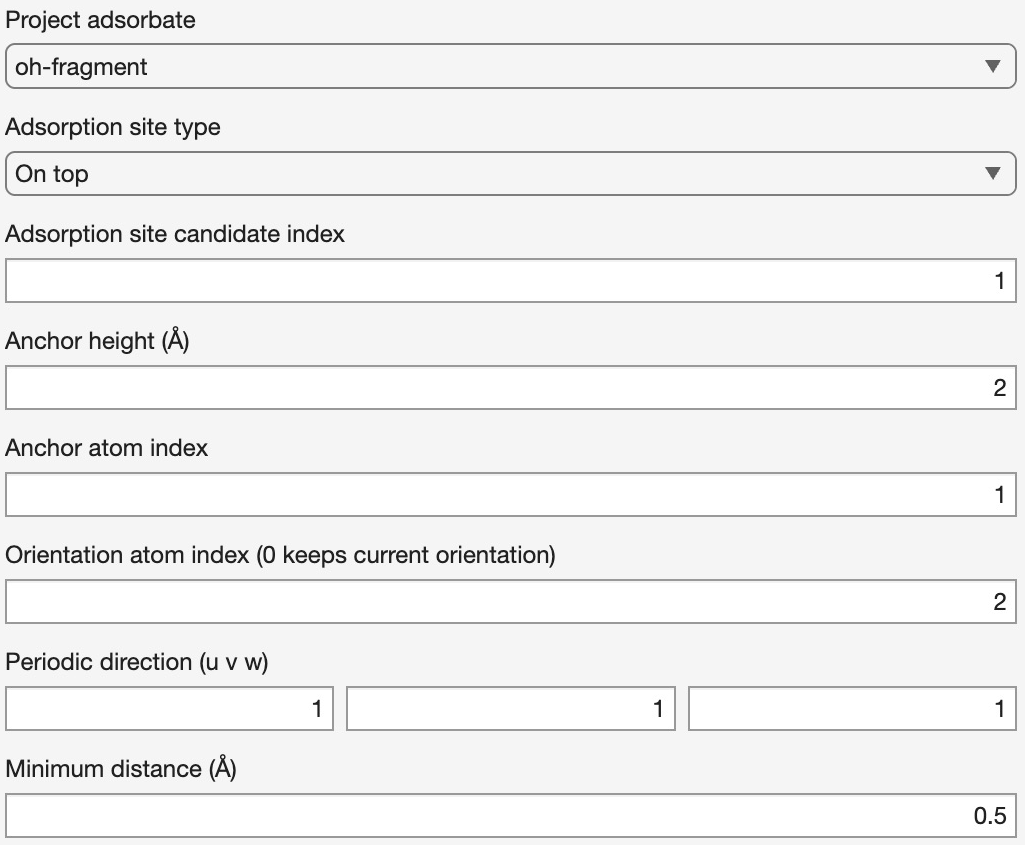
\includegraphics[width=107mm]{publication-assets/crop-c02e14aa8762e8947bbe.png}
\caption{Outward O--H placement: project fragment \file{oh-fragment}, ontop candidate 1, anchor height $2\,\text{\AA}$, anchor atom 1, orientation atom 2, periodic-direction indices 1, 1, 1, and minimum separation $0.5\,\text{\AA}$. The host $c$ vector is first aligned with the surface normal.}
\label{fig:pt111-oh-parameters}
\end{figure}

\begin{figure}[H]
\centering
\begin{minipage}[t]{80mm}
\vspace{0pt}
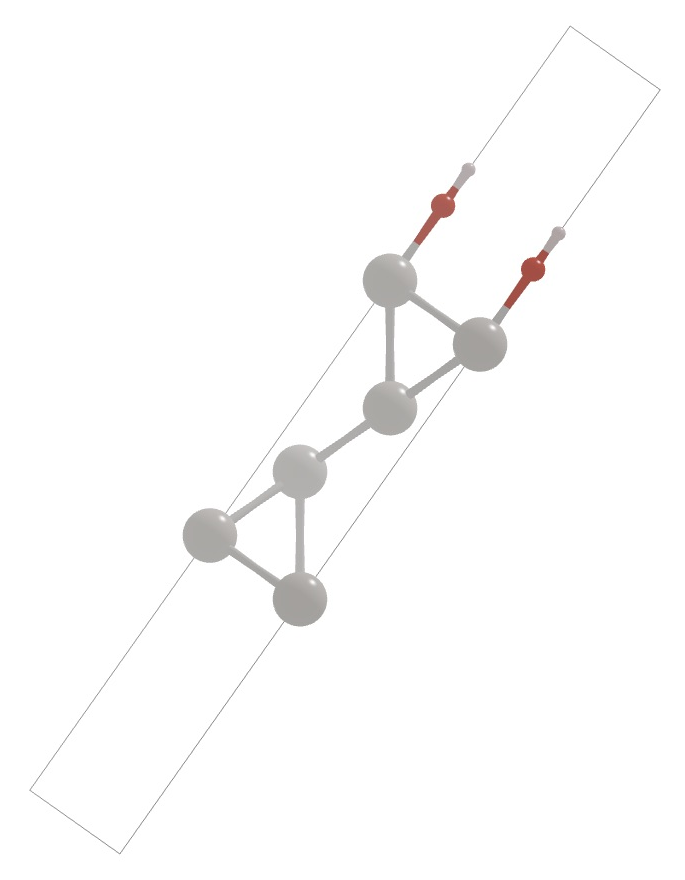
\includegraphics[width=\linewidth]{publication-assets/crop-c201c0495d5d847c2fd3.png}
\end{minipage}\hfill
\begin{minipage}[t]{40mm}
\vspace{0pt}
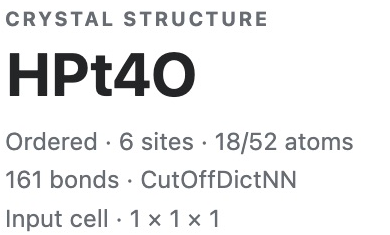
\includegraphics[width=\linewidth]{publication-assets/crop-5caa5064e4762ffc4974.png}
\end{minipage}
\caption{Side view after applying adsorption placement and wrapping with a $1\times1\times1$ unit supercell. The $\mathrm{Pt_4OH}$ model has 6 independent sites. The two displayed O--H groups are periodic images of one fragment. This is the initial placed geometry.}
\label{fig:pt111-oh-side}
\end{figure}
